\chapter{Another zedboard} 
\label{ch:anotherzedboard} 

We changed board and the bootloader started well without giving the stackoverflow error but randomly didn’t start.\\
After having tried the same parameters previously inserted, the bootloader couldn’t  initialize inet and some network settings.

\begin{figure}[h]
	\centering		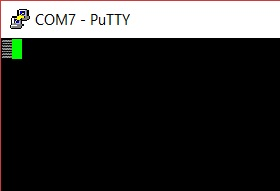
\includegraphics[width=0.6\textwidth]{img/error1}
	\caption{Error}
    	\label{fig:error1}
\end{figure}

\begin{figure}[h]
	\centering		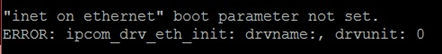
\includegraphics[width=0.6\textwidth]{img/error2}
	\caption{Another error}
    	\label{fig:error2}
\end{figure}

\section{Wrong kernel image}

Following this guide 
\href{https://www.xilinx.com/support/documentation/application_notes/xapp1258-vxworks-7-bsp.pdf}{Guide}
we tried to boot the vxWorks image but it can’t get the kernel image.
\begin{figure}[h]
	\centering		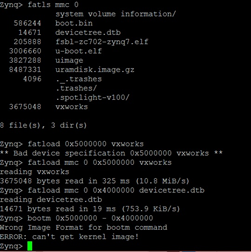
\includegraphics[width=0.4\textwidth]{img/error3}
	\caption{Wrong kernel image}
    	\label{fig:error3}
\end{figure}

\section{U-BOOT}
We rebuilded the image following the configurations parameters provided by the guide  but we had the same error.

\begin{figure}[h]
	\centering		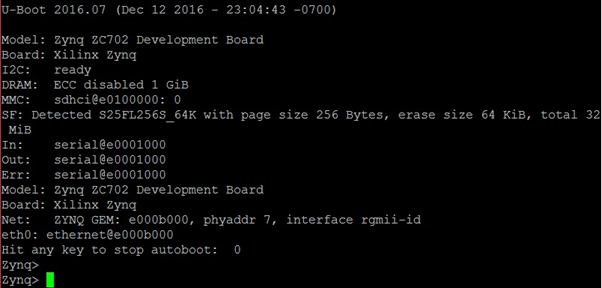
\includegraphics[width=0.6\textwidth]{img/error4}
	\caption{Boot problem}
    	\label{fig:error4}
\end{figure}




